\documentclass[journal,12pt,twocolumn]{IEEEtran}

\usepackage{setspace}
\usepackage{paralist}
\usepackage{gensymb}
\singlespacing
\usepackage[cmex10]{amsmath}

\usepackage{amsthm}
\usepackage{amssymb}

\usepackage{mathrsfs}
\usepackage{txfonts}
\usepackage{stfloats}
\usepackage{bm}
\usepackage{cite}
\usepackage{cases}
\usepackage{subfig}

\usepackage{longtable}
\usepackage{multirow}

\usepackage{enumitem}
\usepackage{mathtools}
\usepackage{steinmetz}
\usepackage{tikz}
\usepackage{circuitikz}
\usepackage{verbatim}
\usepackage{tfrupee}
\usepackage[breaklinks=true]{hyperref}
\usepackage{graphicx}
\usepackage{tkz-euclide}

\usetikzlibrary{calc,math}
\usepackage{listings}
    \usepackage{color}                                            %%
    \usepackage{array}                                            %%
    \usepackage{longtable}                                        %%
    \usepackage{calc}                                             %%
    \usepackage{multirow}                                         %%
    \usepackage{hhline}                                           %%
    \usepackage{ifthen}                                           %%
    \usepackage{lscape}     
\usepackage{multicol}
\usepackage{chngcntr}
\usepackage{mathtools}
\DeclarePairedDelimiter\ceil{\lceil}{\rceil}
\DeclarePairedDelimiter\floor{\lfloor}{\rfloor}

\DeclareMathOperator*{\Res}{Res}

\renewcommand\thesection{\arabic{section}}
\renewcommand\thesubsection{\thesection.\arabic{subsection}}
\renewcommand\thesubsubsection{\thesubsection.\arabic{subsubsection}}

\renewcommand\thesectiondis{\arabic{section}}
\renewcommand\thesubsectiondis{\thesectiondis.\arabic{subsection}}
\renewcommand\thesubsubsectiondis{\thesubsectiondis.\arabic{subsubsection}}


\hyphenation{op-tical net-works semi-conduc-tor}
\def\inputGnumericTable{}                                 %%

\lstset{
%language=C,
frame=single, 
breaklines=true,
columns=fullflexible
}
\begin{document}

\newcommand{\BEQA}{\begin{eqnarray}}
\newcommand{\EEQA}{\end{eqnarray}}
\newcommand{\define}{\stackrel{\triangle}{=}}
\bibliographystyle{IEEEtran}
\raggedbottom
\setlength{\parindent}{0pt}
\providecommand{\mbf}{\mathbf}
\providecommand{\pr}[1]{\ensuremath{\Pr\left(#1\right)}}
\providecommand{\qfunc}[1]{\ensuremath{Q\left(#1\right)}}
\providecommand{\sbrak}[1]{\ensuremath{{}\left[#1\right]}}
\providecommand{\lsbrak}[1]{\ensuremath{{}\left[#1\right.}}
\providecommand{\rsbrak}[1]{\ensuremath{{}\left.#1\right]}}
\providecommand{\brak}[1]{\ensuremath{\left(#1\right)}}
\providecommand{\lbrak}[1]{\ensuremath{\left(#1\right.}}
\providecommand{\rbrak}[1]{\ensuremath{\left.#1\right)}}
\providecommand{\cbrak}[1]{\ensuremath{\left\{#1\right\}}}
\providecommand{\lcbrak}[1]{\ensuremath{\left\{#1\right.}}
\providecommand{\rcbrak}[1]{\ensuremath{\left.#1\right\}}}
\theoremstyle{remark}
\newtheorem{rem}{Remark}
\newcommand{\sgn}{\mathop{\mathrm{sgn}}}
\providecommand{\abs}[1]{\vert#1\vert}
\providecommand{\res}[1]{\Res\displaylimits_{#1}} 
\providecommand{\norm}[1]{\lVert#1\rVert}
%\providecommand{\norm}[1]{\lVert#1\rVert}
\providecommand{\mtx}[1]{\mathbf{#1}}
\providecommand{\mean}[1]{E[ #1 ]}
\providecommand{\fourier}{\overset{\mathcal{F}}{ \rightleftharpoons}}
%\providecommand{\hilbert}{\overset{\mathcal{H}}{ \rightleftharpoons}}
\providecommand{\system}{\overset{\mathcal{H}}{ \longleftrightarrow}}
	%\newcommand{\solution}[2]{\textbf{Solution:}{#1}}
\newcommand{\solution}{\noindent \textbf{Solution: }}
\newcommand{\cosec}{\,\text{cosec}\,}
\providecommand{\dec}[2]{\ensuremath{\overset{#1}{\underset{#2}{\gtrless}}}}
\newcommand{\myvec}[1]{\ensuremath{\begin{pmatrix}#1\end{pmatrix}}}
\newcommand{\mydet}[1]{\ensuremath{\begin{vmatrix}#1\end{vmatrix}}}
\numberwithin{equation}{subsection}
\makeatletter
\@addtoreset{figure}{problem}
\makeatother
\let\StandardTheFigure\thefigure
\let\vec\mathbf
\renewcommand{\thefigure}{\theproblem}
\def\putbox#1#2#3{\makebox[0in][l]{\makebox[#1][l]{}\raisebox{\baselineskip}[0in][0in]{\raisebox{#2}[0in][0in]{#3}}}}
     \def\rightbox#1{\makebox[0in][r]{#1}}
     \def\centbox#1{\makebox[0in]{#1}}
     \def\topbox#1{\raisebox{-\baselineskip}[0in][0in]{#1}}
     \def\midbox#1{\raisebox{-0.5\baselineskip}[0in][0in]{#1}}
\vspace{3cm}
\title{\textbf{AI1103 : Assignment 5}}
\author{\textbf{Santosh Dhaladhuli MS20BTECH11007}}
\maketitle
\newpage
\bigskip
\renewcommand{\thefigure}{\theenumi}
\renewcommand{\thetable}{\theenumi}

Download all python codes from 
\begin{lstlisting}
https://github.com/Santosh-Dhaladhuli2003/AI1103/blob/main/Assignment%205/Assignment%205.py
\end{lstlisting}
%
and latex codes from 
%
\begin{lstlisting}
https://github.com/Santosh-Dhaladhuli2003/AI1103/blob/main/Assignment%205/Assignment%205.tex
\end{lstlisting}
\section{\textbf{GATE IN 2007 Question No. 27}}
Assume that the duration in minutes of a telephone conversation follows the exponential distribution f(x) = $\frac{1}{5}e^{-\frac{x}{5}}$, x $\ge$ 0. The probability that the conversation will exceed five minutes is...

\begin{enumerate}
\item $\frac{1}{e}$ 
\item 1 - $\frac{1}{e}$ 
\item $\frac{1}{e^2}$ 
\item 1 - $\frac{1}{e^2}$
\end{enumerate}

\section{\textbf{Solution}}
Let X be a Random variable defined,that denotes the duration of a telephonic conversation in minutes.\\
So, X $\in$ [0,$\infty$) \\
Given, f$_X$(x) = $\frac{1}{5}e^{-\frac{x}{5}}$ \\
Let CDF of X be F$_X$(x)
\begin{align*}
F_X(x) &=  \int_{-\infty}^{x}f_X(t) \,dt \\
       &= \int_{-\infty}^{0}f_X(t) \,dt + \int_{0}^{x}f_X(t) \,dt \\
F_X(x) &= \int_{0}^{x}f_X(t) \,dt  \because f_X(x) = 0 \forall x<0  \\
\therefore F_X(x) &= \int_{0}^{x}\frac{1}{5}e^{-\frac{t}{5}} \,dt \\
\tag{1}
\label{CDF}
\implies F_X(x) &= 1 - e^{-\frac{x}{5}}
\end{align*}
\begin{align*}
\text{We Know } F_X(x) &= \pr{X \le x} \\
\text{Required Probability is }\pr{X > 5} &= 1 - \pr{X \le 5} \\
\implies \pr{X > 5} &= 1 - F_X(5) \\
 &= 1 - (1 - e^{-\frac{5}{5}}) \\
 &= e^{-\frac{5}{5}}  \\
 &= e^{-1} = \frac{1}{e}
\end{align*}
$\therefore$ The correct answer is \textbf{Option 1}
\begin{figure}[!htb]
    \centering
    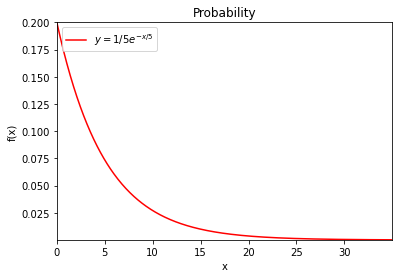
\includegraphics[width = 0.45\textwidth]{Exp Assignment 5.png}
    \label{EXP}
\end{figure}
\begin{figure}[!htb]
    \centering
    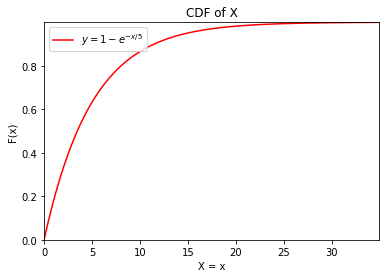
\includegraphics[width = 0.45\textwidth]{CDF assignment 5.png}
    \label{cdf}
\end{figure}
\end{document}
